\documentclass{beamer}
\usepackage{listings,hyperref,graphicx,amsmath,animate,tikz}
\usetikzlibrary{positioning,shadows,arrows,shapes,calc}
\def\labelenumi\theenumi
\mode<presentation>{\usetheme{Frankfurt}}
\AtBeginSection
{
  \begin{frame}<beamer>
    \frametitle{Outline}
    \tableofcontents[currentsection,currentsubsection]
  \end{frame}
}
\title{Lecture 2: SVD, Pseudo-Inverse, and Projection}
\author{Mark Hasegawa-Johnson\\These slides are in the public domain.}
\date{ECE 417: Multimedia Signal Processing, Fall 2023}  
\institute{University of Illinois}
\titlegraphic{\includegraphics[width=0.3in]{exp/block-I-primary.png}}
\begin{document}

% Title
\begin{frame}
  \maketitle
\end{frame}

% Title
\begin{frame}
  \tableofcontents
\end{frame}

%%%%%%%%%%%%%%%%%%%%%%%%%%%%%%%%%%%%%%%%%%%%%%%%%%%%%%%%%
\section{Application: Animating a still image}
\setcounter{subsection}{1}

\begin{frame}
  \frametitle{Input \#1: X-Ray Microbeam Data}
  \centerline{\animategraphics[loop,controls,height=2.5in]{20}{exp/mp1_xrmb_movie-}{0}{42}}
\end{frame}

\begin{frame}
  \frametitle{Input \#2: A Still Image Acquired Using MRI}
  \centerline{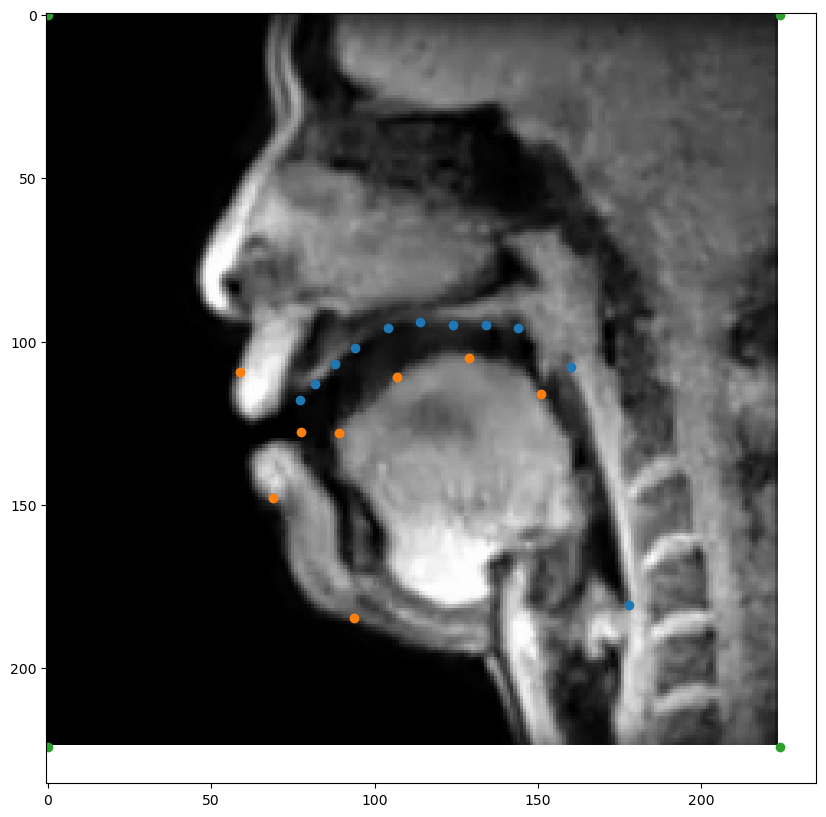
\includegraphics[height=2.5in]{mp1_mri_points.png}}
\end{frame}

\begin{frame}
  \frametitle{Desired Output: Animated Image}
  \centerline{\animategraphics[loop,controls,height=2.5in]{20}{exp/mp1_result-}{0}{42}}
\end{frame}

\begin{frame}
  \frametitle{Strategy}
  \begin{enumerate}
  \item Use affine projection to rotate, scale, and shear the XRMB
    points so that they match the shape of the MRI as well as possible.
  \item Draw triangles on the MRI so that every pixel is inside a triangle.
  \item Move the triangles.
  \end{enumerate}
\end{frame}

\begin{frame}
  \frametitle{Step 1 (Today): Use affine projection to map XRMB to MRI}
  \centerline{\animategraphics[loop,controls,height=2.5in]{20}{exp/mp1_procrustes_movie-}{0}{42}}
\end{frame}

\begin{frame}
  \frametitle{Step 2 (Next time): Draw triangles on the MRI}
  \centerline{\animategraphics[loop,controls,height=2.5in]{20}{exp/mp1_procrustes_triangles-}{0}{42}}
\end{frame}

%%%%%%%%%%%%%%%%%%%%%%%%%%%%%%%%%%%%%%%%%%%%%%%%%%%%%%%%%
\section{Singular Value Decomposition}
\setcounter{subsection}{1}

\begin{frame}
  \frametitle{Summary: Purpose of this section}

  Any real-valued matrix of any dimension, $M\in\Re^{m\times n}$, can
  be written as
  \[
  M = U\Sigma V^T
  \]
  \ldots where $\Sigma$ is a diagonal matrix, and $U$ and $V$ are
  orthonormal matrices.
\end{frame}

\begin{frame}
  \frametitle{Proof Step \#1: Eigenvectors of a Gram Matrix}

  The gram matrix, $G=M^TM\in\Re^{n\times n}$, is the matrix whose
  elements are inner products between the {\bf columns} of $M$.  $G$
  is square, symmetric, and positive-semidefinite, therefore
  $G=V\Lambda V^T$, where
  \begin{align*}
    V=\left[v_1,\ldots,v_n\right],~~~
    &\Lambda=\left[\begin{array}{cccc}\lambda_1&0&\cdots&0\\
        0&\lambda_2&\cdots&0\\\vdots&\vdots&\ddots&0\\
        0&0&\cdots&\lambda_n
      \end{array}\right]
  \end{align*}
  \begin{itemize}
  \item The rows and columns of $V$ are orthonormal, $VV^T=V^TV=I$
  \item $\lambda_i\ge 0$ are the eigenvalues of $G$
  \end{itemize}
\end{frame}

\begin{frame}
  \frametitle{Proof Step \#2: Singular Values}

  The eigenvalues are non-negative, so we can take their square roots:
  \begin{align*}
    \Sigma &= \Lambda^{1/2}\\ 
    &=\left[\begin{array}{cccc}\sigma_1&0&\cdots&0\\
        0&\sigma_2&\cdots&0\\\vdots&\vdots&\ddots&0\\
        0&0&\cdots&\sigma_n
      \end{array}\right]
  \end{align*}
  where $\sigma_i=\sqrt{\lambda_i}$.  Therefore, we can write
  \begin{align*}
    G &= V\Lambda V^T = V\Sigma\Sigma V^T
  \end{align*}
\end{frame}

\begin{frame}
  \frametitle{Proof Step \#3: the Sum-of-Squares Matrix}
  The sum-of-squares matrix, $S=MM^T\in\Re^{m\times m}$, is the matrix whose
  elements are inner products between the {\bf rows} of $M$.  $S$
  is square, symmetric, and positive-semidefinite, therefore
  $S=U\Lambda U^T$, where
  \begin{align*}
    U=\left[u_1,\ldots,u_m\right],~~~
    &\Lambda=\left[\begin{array}{cccc}\lambda_1&0&\cdots&0\\
        0&\lambda_2&\cdots&0\\\vdots&\vdots&\ddots&0\\
        0&0&\cdots&\lambda_m
      \end{array}\right]
  \end{align*}
  \begin{itemize}
  \item The eigenvalues of $S$ are the same as the eigenvalues of $G$, except that
    if $m>n$, the extra eigenvalues are all zero: $\lambda_{n+1}=\cdots=\lambda_m=0$.
  \item The rows and columns of $U$ are orthonormal, $UU^T=U^TU=I$
  \end{itemize}
\end{frame}

\begin{frame}
  \frametitle{Proof Step \#4: Replace $I$ by $U^TU$}

  Starting with $G=VSSV^T$, we can introduce an identity matrix into
  the middle to get
  \begin{displaymath}
    G = V\Sigma I\Sigma V^T = V\Sigma U^TU\Sigma V^T
  \end{displaymath}
  But by the same logic, we can write
  \begin{displaymath}
    S = U\Sigma I\Sigma U^T = U\Sigma V^TV\Sigma U^T
  \end{displaymath}
  The only way these can both be true is if the original matrix was
  \begin{displaymath}
    M = U\Sigma V^T
  \end{displaymath}
\end{frame}

\begin{frame}
  \begin{columns}[t]
    \column{2.5in}
    \begin{block}{Singular Value Decomposition}
      Any real matrix $M\in\Re^{m\times n}$ can be decomposed as
      \[
      M=U\Sigma V^T
      \]
    \end{block}
    \column{2.25in}
    \begin{block}{}
      \centerline{\includegraphics[width=2.25in]{exp/SVD_visualization.png}}
      \centerline{\tiny\href{https://en.wikipedia.org/wiki/Singular_value_decomposition}{CC-SA 4.0, Cmglee}}
    \end{block}
  \end{columns}
\end{frame}

%%%%%%%%%%%%%%%%%%%%%%%%%%%%%%%%%%%%%%%%%%%%%%%%%%%%%%%%%
\section{Pseudo-Inverse}
\setcounter{subsection}{1}

\begin{frame}
  \frametitle{Summary: Purpose of this section}

  Any arbitrary real matrix $M=U\Sigma V^T\in\Re^{m\times n}$ has a
  pseudo-inverse, defined as
  \begin{displaymath}
    M^\dag = U_r\Sigma_r^{-1} V_r^T
  \end{displaymath}
  where $U_r$, $\Sigma_r$, and $V_r$ are the ``compact singular value
  decomposition'' of $M$, defined as:
  \begin{itemize}
  \item $\Sigma_r\in\Re^{r\times r}$ contains only the nonzero singular values,
  \item $U_r\in\Re^{m\times r}$ contains the corresponding columns of $U$,
  \item $V_r\in\Re^{n\times r}$ contains the corresponding columns of $V$.
  \end{itemize}
\end{frame}
  
\begin{frame}
  \frametitle{Why it makes sense: Eigenvalue definition of matrix inverse}

  First, suppose that $G$ is a square positive-definite matrix, i.e.,
  all of its eigenvalues are greater than zero.  Then we can write
  $G$-inverse as
  \begin{align*}
    G^{-1} = V\Lambda^{-1}V^T
  \end{align*}
  Proof:
  \begin{align*}
    G^{-1}G &= \left(V\Lambda^{-1}V^T\right)\left(V\Lambda V^T\right)\\
    &= V\Lambda^{-1}\Lambda V^T\\
    &= VV^T\\
    &= I
  \end{align*}
\end{frame}

\begin{frame}
  \frametitle{Algebraic Forms}

  \begin{itemize}
  \item If $m<n$ and $M$ has full row rank (all rows linearly
    independent), then $MM^T\in\Re^{m\times m}$ is invertible, and
    \begin{displaymath}
      M^\dag = M^T(MM^T)^{-1}
    \end{displaymath}
  \item If $m>n$ and $M$ has full column rank (all columns linearly
    independent), then $M^TM\in\Re^{n\times n}$ is invertible, and
    \begin{displaymath}
      M^\dag = (M^TM)^{-1} M^T
    \end{displaymath}
  \end{itemize}
  The homework will explore the properties of these two very useful special cases.
\end{frame}

\begin{frame}
  \frametitle{Proof that the Algebraic Forms are Pseudo-Inverse}

  Suppose that $M=U_r\Sigma_r V_r^T$, and $M^\dag = U_r\Sigma_r^{-1}
  V_r^T$.  Then
  \begin{align*}
    M^T(MM^T)^{-1} &= V_r\Sigma_rU_r^T(U_r\Sigma_rV_r^TV_r\Sigma_rU_r^T)^{-1}\\
    &= V_r\Sigma_rU_r^T(U_r\Sigma_r\Sigma_rU_r^T)^{-1}\\
    &= V_r\Sigma_rU_r^T(U_r\Lambda_rU_r^T)^{-1}\\
    &= V_r\Sigma_rU_r^TU_r\Lambda_r^{-1}U_r^T\\
    &= V_r\Sigma_r\Lambda_r^{-1}U_r^T\\
    &= V_r\Sigma_r^{-1}U_r^T\\
    &= M^\dag
  \end{align*}
\end{frame}

%%%%%%%%%%%%%%%%%%%%%%%%%%%%%%%%%%%%%%%%%%%%%%%%%%%%%%%%%
\section{Affine Transformations}
\setcounter{subsection}{1}

\begin{frame}
  \frametitle{Affine Transformation}

  Given an input pixel location
  $x=\left[\begin{array}{c}x_1\\x_2\end{array}\right]\in\Re^2$, the
  goal is to rotate, scale, shift and shear the image to find an
  output pixel location
  $u=\left[\begin{array}{c}u_1\\u_2\end{array}\right]\in\Re^2$.

  An {\bf affine transform} is a linear transform plus a shift:
  \[
  \left[\begin{array}{c} u_1\\u_2\end{array}\right]=
  \left[\begin{array}{cc}a_{1,1}&a_{1,2}\\a_{2,1}&a_{2,2}\end{array}\right]
  \left[\begin{array}{c}x_1\\x_2\end{array}\right] +
  \left[\begin{array}{c}b_1\\b_2\end{array}\right]
  \]
  \ldots or we could just write\ldots
  \[
  u = Ax+b
  \]
\end{frame}
  
\begin{frame}
  \frametitle{Affine Transforms}

  Notice that the affine transformation has 6 degrees of freedom:
  $(a_{1,1},a_{1,2},a_{2,1},a_{2,2},b_1,b_2)$.  Therefore, you can
  accmplish 6 different types of transformation:
  \begin{itemize}
  \item Shift the image left$\leftrightarrow$right (using $b_1$)
  \item Shift the image up$\leftrightarrow$down (using $b_2$)
  \item Scale the image horizontally (using $a_{1,1}$)
  \item Scale the image vertically (using $a_{2,2}$)
  \item Rotate the image (using $a_{1,1},a_{1,2},a_{2,1},a_{2,2}$)
  \item Shear the image horizontally (using $a_{1,2}$)
  \end{itemize}
  Vertical shear (using $a_{2,1}$) is a combination of horizontal shear + rotation.
\end{frame}

\begin{frame}
  \frametitle{Example: Reflection}
  \centerline{\includegraphics[height=2in]{exp/Checkerboard_identity.png}\includegraphics[height=2in]{exp/Checkerboard_reflection.png}}
  \centerline{\small CC-SA 4.0, \url{https://en.wikipedia.org/wiki/Affine_transformation}}
  \[
  \left[\begin{array}{c} u\\v\\1\end{array}\right]=
  \left[\begin{array}{ccc}-1&0&0\\0&1&0\\0&0&1\end{array}\right]
  \left[\begin{array}{c}x\\y\\1\end{array}\right]
  \]
\end{frame}

\begin{frame}
  \frametitle{Example: Scale}
  \centerline{\includegraphics[height=2in]{exp/Checkerboard_identity.png}\includegraphics[height=2in]{exp/Checkerboard_scale.png}}
  \centerline{\small CC-SA 4.0, \url{https://en.wikipedia.org/wiki/Affine_transformation}}
  \[
  \left[\begin{array}{c} u\\v\\1\end{array}\right]=
  \left[\begin{array}{ccc}2&0&0\\0&1&0\\0&0&1\end{array}\right]
  \left[\begin{array}{c}x\\y\\1\end{array}\right]
  \]
\end{frame}

\begin{frame}
  \frametitle{Example: Rotation}
  \centerline{\includegraphics[height=2in]{exp/Checkerboard_identity.png}\includegraphics[height=2in]{exp/Checkerboard_rotate.png}}
  \centerline{\small CC-SA 4.0, \url{https://en.wikipedia.org/wiki/Affine_transformation}}
  \[
  \left[\begin{array}{c} u\\v\\1\end{array}\right]=
  \left[\begin{array}{ccc}\cos\theta&-\sin\theta&0\\\sin\theta&\cos\theta&0\\0&0&1\end{array}\right]
  \left[\begin{array}{c}x\\y\\1\end{array}\right]
  \]
\end{frame}

\begin{frame}
  \frametitle{Example: Shear}
  \centerline{\includegraphics[height=2in]{exp/Checkerboard_identity.png}\includegraphics[height=2in]{exp/Checkerboard_shear.png}}
  \centerline{\small CC-SA 4.0, \url{https://en.wikipedia.org/wiki/Affine_transformation}}
  \[
  \left[\begin{array}{c} u\\v\\1\end{array}\right]=
  \left[\begin{array}{ccc}1&0.5&0\\0&1&0\\0&0&1\end{array}\right]
  \left[\begin{array}{c}x\\y\\1\end{array}\right]
  \]
\end{frame}

%%%%%%%%%%%%%%%%%%%%%%%%%%%%%%%%%%%%%%%%%%%%%%%%%%%%%%%%%
\section{MMSE Estimation of an Affine Transform}
\setcounter{subsection}{1}

\begin{frame}
  \begin{columns}[t]
    \column{2.5in}
    \begin{block}{Input}
      Suppose we have a set of points like this:
      \centerline{\animategraphics[loop,controls,height=2.5in]{20}{exp/mp1_xrmb_movie-}{0}{42}}
    \end{block}
    \column{2.25in}
    \begin{block}{Output}
      ...we want to rotate, reflect, shift and scale so it looks like
      this:
      \centerline{\animategraphics[loop,controls,height=2.5in]{20}{exp/mp1_procrustes_movie-}{0}{42}}
    \end{block}
  \end{columns}
\end{frame}

\begin{frame}
  \frametitle{Estimating an Affine Transform}

  Our goal is to find a $3\times 2$ affine transform matrix, $A$, such that
  \begin{displaymath}
    Y\approx XA
  \end{displaymath}
  where $x_i=[x_{i,1},x_{i,2},1]$ is a 1-augmented X-ray microbeam
  landmark point, $y_i=[y_{i,1},y_{i,2}]$ is the corresponding MRI
  landmark point, and
  \begin{displaymath}
    Y=\left[\begin{array}{cc}
        y_{1,1}&y_{2,1}\\
        \vdots&\vdots\\
        y_{n,1}&y_{n,1}
      \end{array}\right],~~~
    X=\left[\begin{array}{ccc}
        x_{1,1}&x_{2,1}&1\\
        \vdots&\vdots&\vdots\\
        x_{n,1}&x_{n,1}&1
      \end{array}\right],~~~
    A=\left[\begin{array}{cc}
        a_{1,1}&a_{1,2}\\
        a_{2,1}&a_{2,2}\\
        b_1&b_2\end{array}\right]
  \end{displaymath}
\end{frame}
    
\begin{frame}
  \frametitle{MMSE Estimation of Affine Transform}

  In particular, suppose we want to minimize the mean-squared error:
  \begin{displaymath}
    \epsilon = \sum_{i=1}^n\Vert x_iA-y_i\Vert^2=\sum_{i=1}^n(x_iA-y_i)(x_iA-y_i)^T
  \end{displaymath}
  Notice that this is just squaring the samples of $XA-Y$, and adding
  across the rows.  That's called the ``Frobenius norm'' of $XA-Y$,
  and there a few different ways it can be expanded:
  \begin{align*}
    \epsilon &= \Vert XA-Y\Vert_F^2\\
    &=\text{trace}\left((XA-Y)(XA-Y)^T\right)\\
    &=\text{trace}\left((XA-Y)^T(XA-Y)\right)\\
  \end{align*}
\end{frame}

\begin{frame}
  \frametitle{MMSE Estimation of Affine Transform}

  Since MMSE is quadratic, we can find the minimum by just
  differentiating with respect to the elements of the matrix.
  Differentiating is easy if we choose the version of $\epsilon$, from
  the previous slide, that puts $A$ on the outside:
  \begin{align*}
    \frac{d\epsilon}{dA} &\equiv
    \left[\begin{array}{cc}
        \frac{d\epsilon}{da_{1,1}} &\frac{d\epsilon}{da_{1,2}}\\
        \frac{d\epsilon}{da_{2,1}} &\frac{d\epsilon}{da_{2,2}}\\
        \frac{d\epsilon}{db_{1}} &\frac{d\epsilon}{db_{2}}
      \end{array}\right]\\
    &=\frac{d}{dA} \text{trace}\left(A^TX^TXA-Y^TXA-A^TX^TY+Y^TY\right)\\
    &= A^TX^TX + (X^TXA)^T -(Y^TX)^T - X^TY
  \end{align*}
  Setting that to zero, we find that the MMSE value of $A$ is
  \begin{displaymath}
    A_{\text{MMSE}} = (X^TX)^{-1}X^TY = X^\dag Y
  \end{displaymath}
\end{frame}

\begin{frame}
  \frametitle{Interpretation of MMSE as Projection}

  Pay attention to what's happening here. $A_{\text{MMSE}} = (X^TX)^{-1}X^TY$, where
  \begin{align*}
    &X^TY=
    &
    %\left[\begin{array}{ccc}
    %    \sum_{i=1}^nx_{i,1}^2&\sum_{i=1}^nx_{i,1}x_{i,2}&\sum_{i=1}^nx_{i,1}\\
    %    \sum_{i=1}^nx_{i,1}x_{i,2}&\sum_{i=1}^nx_{i,2}^2&\sum_{i=1}^nx_{i,2}\\
    %    \sum_{i=1}^nx_{i,1}&\sum_{i=1}^nx_{i,2}&n
    %  \end{array}\right]^{-1}
    \left[\begin{array}{cccc}
        x_{1,1}&x_{2,1}&\cdots&x_{n,1}\\
        x_{1,2}&x_{2,2}&\cdots&x_{n,2}\\
        1&1&\cdots&1
      \end{array}\right]
    \left[\begin{array}{cc}
        y_{1,1}&y_{2,1}\\
        \vdots&\vdots\\
        y_{n,1}&y_{n,1}
      \end{array}\right]
  \end{align*}
  So $A_{\text{MMSE}}$ projects each column of $Y$ onto the columns of $X$, then
  normalizes by $(X^TX)^{-1}$.
\end{frame}

\begin{frame}
  \begin{columns}[t]
    \column{2.5in}
    \begin{block}{Interpreting MMSE as Projection}
      If $X$ is tall and thin, columns of $Y$ are projected onto
      columns of $X$ as
      \begin{align*}
        \hat{Y}&=X(X^TX)^{-1}X^TY\\
        &=XX^\dag Y
      \end{align*}
      If $X$ is short and fat, columns of $Y$ are projected onto
      {\bf rows} of $X$ as
      \begin{align*}
        \hat{Y}&=X^T(XX^T)^{-1}XY\\
        &=X^\dag XY
      \end{align*}
    \end{block}
    \column{2.25in}
    \begin{block}{}
      \centerline{\includegraphics[width=\textwidth]{exp/Ortho_projection.png}}
    \end{block}
  \end{columns}
\end{frame}

    
%%%%%%%%%%%%%%%%%%%%%%%%%%%%%%%%%%%%%%%%%%%%%%%%%%%%%%%%%
\section{Conclusions}
\setcounter{subsection}{1}
\begin{frame}
  \frametitle{Conclusions}
  \begin{itemize}
  \item Singular value decomposition:
    \begin{displaymath}
      M = U\Sigma V^T = U_r\Sigma_rV_r^T
    \end{displaymath}
  \item Pseudo-inverse:
    \begin{align*}
      M^\dag &= U_r\Sigma_r^{-1}V_r^T\\
      &= (M^TM)^{-1}M^T~~\text{if}~M~\text{tall \& thin}\\
      &= M^T(MM^T)^{-1}~~\text{if}~M~\text{short \& fat}
    \end{align*}
  \item MMSE Projection:
    \begin{displaymath}
      A_{\text{MMSE}}=(X^TX)^{-1}X^TY
    \end{displaymath}
  \end{itemize}
\end{frame}
\end{document}

